\chapter{Создаем переиспользуемые компоненты}

Для того чтобы создавать действительно переиспользуемые компоненты мы должны разобраться, какие в целом способы создания компонент предоставляет React и какой в каком случае стоит выбирать. Также относительно недавно в React появился новая способ определения компонент с помощью \textbf{безстейтовых функций (stateless function)}

Один из способов изучения - рассмотреть множество примеров. Следуя по этому пути, мы начнем с примера компонента, который имеет узкую специализацию, и превратим его в переиспользуемый.

В этой главе мы рассмотрим:

\begin{itemize}
  \item Различные способы создания React компонент и когда какие из них следует использовать
  \item Что такое stateless компоненты и чем они отличаются от stateful компонент
  \item Как работает state компонент и когда следует избежать его использование
  \item Почему важно определять prop types для каждого компоненты и как с помощью них создавать динамически документацию с помощью \textbf{React Docgen}
  \item Примеры создания универсальных компонент из узкоспециализированных
  \item Как мы можем задокументировать нашу коллекцию универсальных компонент с помощью \textbf{React Storybook}
\end{itemize}


\section{Создание классов}

Давайте начнем детально разбираться с возможностями определения компонент, которые предоставляет React.

\subsection*{Фабрика createClass}

Если открыть документацию React, то первый способ создания компонента, который мы найдем, будет $React.createClass$.

Попробуем создать с его помощью простой пример:

\begin{lstlisting}
const Button = React.createClass({
  render() {
    return <button />
  },
})
\end{lstlisting}

Мы создали простую кнопку, которую можем использовать внутри других компонент нашего приложения.

Мы даже можем заменить JSX внутри этого компонента на обычный JavaScript:

\begin{lstlisting}
const Button = React.createClass({
  render() {
    return React.createElement('button')
  },
})
\end{lstlisting}

Теперь нам не придется использовать babel для запуска этого кода, что значит, что мы можем открыть его напрямую в браузере.

\subsection*{Наследование React.Component}

Следующий подход - использовать классы ES2015. Ключевое слово $class$ уже неплохо поддерживается браузерами, но все равно в этом случае уже лучше транслировать код с babel.

Создадим ту же кнопку, но уже с использование JavaScript классов:

\begin{lstlisting}
class Button extends React.Component {
  render() {
    return <button />
  }
}
\end{lstlisting}

Этот способ создание компонент появился с версии React 0.13 и разработчики Facebook настаивают на том, что использоваться должен именно он. Активный участник React сообщества Ден Абрамов (Dan Abramov) в защиту преимущества ES2015 классов перед createClass высказал: 

\textit{"ES6 classes: better the devil that's standardized (Классы ES6: лушче тот дъявол, который стандартизирован)"}

Таким разработчики библиотеки React ратуют за использование стандартных классов ES2015 вместо createClass фабрики. 

\subsection*{Главные отличия}

За исключением синтаксических различий есть значительные различия, которые стоит держать в голове. Давайте взглянем на них, чтобы вы могли осознанно выбирать между ними во время разработки проекта.

\subsubsection*{Props}

Первое различие, которое мы рассмотрим, заключается в том, как мы определяем параметры, которые получает компонент и как мы задаем для них стандартные значение.

Как работает передача параметров компоненту мы рассмотрим чуть позже, сейчас сконцентрируемся на том, как они определяются.

В $createClass$ мы определяется параметры, которые можно передать компоненту, в поле $propTypes$ объекта, передаваемого этой функции, а значения по умолчанию передаем с помощью функции $getDefaultProps$:

\begin{lstlisting}
const Button = React.createClass({
  propTypes: {
    text: React.PropTypes.string,
  },
  getDefaultProps() {
    return {
      text: 'Click me!',
    }
  },
  render() {
    return <button>{this.props.text}</button>
  }, 
})
\end{lstlisting}

Чтобы получить тот же результат с помощью JavaScript классов, нам нужно будет немного поменять структуру:

\begin{lstlisting}
class Button extends React.Component {
  render() {
    return <button>{this.props.text}</button>
  }
}
Button.propTypes = {
  text: React.PropTypes.string,
}
Button.defaultProps = {
  text: 'Click me!',
}
\end{lstlisting}

Мы вынуждены определить $propTypes$ и $defaultProps$ вне класса, так как \textbf{Class Properties} еще не являются частью стандарта языка.

Когда нам нужно определить параметры по умолчанию, нам нужно было возвращать их из специальной функции, с JavaScript классами нам достаточно определить их в параметры класса.

Основной плюс в том, что с использованием классов, мы избавились от специфичных для React функций, таких как $getDefaultProps$.

\subsubsection*{State}

Еще одно различие заключается в том, как мы можем определить начальное состояние компонента.

Аналогично с определением параметров в $createClass$ мы используем функция, а в ES2015 классе атрибут экземпляра класса.

Посмотрим на пример:

\begin{lstlisting}
const Button = React.createClass({
  getInitialState() {
    return {
      text: 'Click me!',
    } 
  },
  render() {
    return <button>{this.state.text}</button>
  }, 
})
\end{lstlisting}

Метод $getInitialState$ должен вернуть объект с начальным состоянием для каждого элемента.

В случае с классом мы должны определить начальное состояние в поле state экземпляра класса, и происходит это в момент вызова конструктора:

\begin{lstlisting}
class Button extends React.Component {
  constructor(props) {
    super(props)
    this.state = {
      text: 'Click me!',
    }
  }
  render() {
    return <button>{this.state.text}</button>
  } 
}
\end{lstlisting}

Два этих способа эквиваленты, единственное, в последнем случае JavaScript классы позволяют нам избавиться от специфичного метода React API.

В ES2015 мы должны также вызвать конструктор родительского класса, чтобы он был проинициализирован и мы могли работать с $this$.

\subsubsection*{Autobinding}

У $createClass$ есть очень удобная фича, которая скрывает механизм работы JavaScript и может вводить в заблуждение начинающих разработчиков. Эта фича позволяет привязывать к компоненту обработчики событий, ожидая, что в момент вызова этого обработчика в $this$ попадет сам компонент.

Подробно об обработчиках событий мы поговорим позднее в \textit{Главе 6}. Сейчас нас интересует только то, как эти обработчики привязываются к компонентам.

Посмотрим на пример:

\begin{lstlisting}
const Button = React.createClass({
  handleClick() {
    console.log(this)
  },
  render() {
    return <button onClick={this.handleClick} />
  }, 
})
\end{lstlisting}

При использовании $createClass$ мы можем спокойно использовать $this$, что позволяет нам использовать другие методы компонента, такие как $this.setState()$. 

Посмотрим, насколько отличается поведение $this$ при наследовании $React.Component$ и как нам добиться такого же поведения. 

Мы можем создать компонент следующим образом:

\begin{lstlisting}
class Button extends React.Component {
  handleClick() {
    console.log(this)
  }
  render() {
    return <button onClick={this.handleClick} />
  } 
}
\end{lstlisting}

Если мы вызовем этот код, то результатом нажатия на кнопку будет $null$. Это связано с тем, что наша функция передается обработчику событий и мы теряем связь с текущим компонентом.

Это не значит, что мы не можем использовать обработчики событий от слова совсем, но нам придется связывать с компонентом вручную.

Разберемся какие есть возможности связывания функций и компонент.

Возможно вы уже знаете, что стрелочные функции ES2015 автоматически связываются с текущим $this$ контекста, где эта функция создается.

Посмотрим на пример стрелочной функции:

\begin{lstlisting}
() => this.setState()
\end{lstlisting}

Если мы транслируем этот код с помощью Babel, то получим:

\begin{lstlisting}
var _this = this;
(function () {
  return _this.setState();
});
\end{lstlisting}

Как вы уже можете догадаться, одно из решений проблемы \textbf{автоматического связывания} - использование стрелочных функций. Посмотрим, как это работает:

\begin{lstlisting}
class Button extends React.Component {
  handleClick() {
    console.log(this)
  }
  render() {
    return <button onClick={() => this.handleClick()} />
  } 
}
\end{lstlisting}

Этот код будет работать корректно. Но у данного варианта есть проблемы с производительностью, чтобы понять почему, нужно разобраться, как этот код работает.

Создание стрелочной функции внутри $render$ метода влечет непредвиденный посторонний эффект. Эта функция пересоздается на каждом вызове $render$, что может происходить довольно часто. 

Помимо того, что мы каждый раз пересоздаем не самый легкий объект функции, мы также передаем этот объект дочерним элементам, заставляя их пересоздаваться.

Лучшим решением будет привязывать эти функции к компоненту в момент вызова конструктора. В этом случае функция и пересоздаваться не будет и будет иметь нужный нам контекст:

\begin{lstlisting}
class Button extends React.Component {
  constructor(props) {
    super(props)
    this.handleClick = this.handleClick.bind(this)
  }
  handleClick() {
    console.log(this)
  }
  render() {
    return <button onClick={this.handleClick} />
  } 
}
\end{lstlisting}

Проблема решена (Прим.пер. помимо этого сейчас можно определить стрелочную функция как параметр класса, тогда она не будет каждый раз пересоздаваться, но и контекст будет иметь правильный):

\begin{lstlisting}
class Button extends React.Component {
  handleClick = () => {
    console.log(this)
  }
  render() {
    return <button onClick={this.handleClick} />
  } 
}
\end{lstlisting}

\subsection*{Stateless functional components}

Есть еще один способ создать компонент, который несколько отличается от первых двух.

Этот способ появился в \textbf{React 0.14} и принес возможности сделать код еще чище.

Чтобы определить компонент, нам достаточно определить функцию, которая будет возвращать React элемент:

\begin{lstlisting}
() => <button />
\end{lstlisting}

Благодаря стрелочной функции этот код минималистичен и понятен. Само собой внутри этой функции можно использовать JSX, иначе бы это, наверно, не имело смысла.

\subsubsection*{Props and context}

Компонент, который не может получить параметры от родительского элемента, в большинстве случаев будет бесполезен. В новом способе определения компонент параметры передаются в первом параметре самой функции:

\begin{lstlisting}
props => <button>{props.text}</button>
\end{lstlisting}

Помимо этого мы можем использовать возможности деструктуризации ES2015:

\begin{lstlisting}
({ text }) => <button>{text}</button>
\end{lstlisting}

Также мы можем определить, какие параметры компонента может принимать, по аналогии с классами через $propTypes$ атрибут самой функции:

\begin{lstlisting}
const Button = ({ text }) => <button>{text}</button>
Button.propTypes = {
  text: React.PropTypes.string,
}
\end{lstlisting}

Также компоненты-функции получают вторым аргументом $контекст (context)$:

\begin{lstlisting}
(props, context) => (
  <button>{context.currency}{props.value}</button>
)
\end{lstlisting}

\subsubsection*{Ключевое слово this}

Главное отличие создания компоненты-функции от других способов определения компонент в том, что в них $this$ не ссылается на сам компонент.

Следствием этого является невозможность управлять жизненным циклом компонента и использовать такие методы как $setState$.

\subsubsection*{State}

Как можно понять из названия (stateless), такие компоненты не обладают внутренним состоянием. 

Все что делает такая компоненты, это принимает параметры и контекст в аргументах функции и возвращает React элемент.

Это напоминает нам о функциональном программировании, в разрезе которого мы можем смотреть на компоненты-функции как на функции React элементов от параметров и контекста.

\subsubsection*{Lifecycle}

Компоненты-функции не предоставляют никаких возможностей по отслеживанию методов жизненного цикла, таких как $componentDidMount$. Все, что не касается непосредственно генерации JSX должно обрабатываться в родительских элементах.

\subsubsection*{Refs and event handlers}

Не смотря на то, что мы не можем получить ссылку на сам элемент, мы все же можем получить ссылки на элементы, которые создаются внутри компонент-функции. Сделать это можно следующим образом:

\begin{lstlisting}
() => {
  let input
  const onClick = () => input.focus()
  return (
    <div>
      <input ref={el => (input = el)} />
      <button onClick={onClick}>Focus</button>
    </div>
  ) 
}
\end{lstlisting}

\subsubsection*{Отсутствие ссылки на компонент}

Еще одно отличие компонент-функций заключается в том, что если мы создадим экземпляр такого компонента с помощью $ReactTestUtils$, мы не получим никакой ссылки на созданный элемент (подробнее о тестировании и отладке мы поговорим в Главе 10).

Например:

\begin{lstlisting}
const Button = React.createClass({
  render() {
    return <button />
  },
})
const component = ReactTestUtils.renderIntoDocument(<Button />)
\end{lstlisting}

В этом случае переменная component содержит ссылку на созданный элемент.

\begin{lstlisting}
const Button = () => <button />
const component = ReactTestUtils.renderIntoDocument(<Button />)
\end{lstlisting}

А в этом случае переменная component будет иметь значение $null$. Для того, чтобы обойти это ограничение, можно обернуть компонент в другой элемент, например $div$:

\begin{lstlisting}
const component = ReactTestUtils.renderIntoDocument(<div><Button/></div>)
\end{lstlisting}

\subsubsection*{Производительность}

Основное, что стоит держать в голове относительно производительности компонент-функций то, что они легковеснее полноценных компонент и лучше поддаются оптимизации внутри самой библиотеки, о чем говорят разработчики Facebook. 

Помимо этого есть нюанс, что в жизненном цикле компонента отсутствует метод $shouldComponentUpdate$, что не дает возможность сказать Reacrt'у, что компонент не нужно повторно вызывать метод render. Это на самая большая проблема, но стоит держать ее в голове.


\section{The state}

Мы разобрались с тем, как создавать компоненты в React.
Теперь мы можем пойти дальше и посмотреть детально на управление состоянием компонент.

Также мы должны понять, когда использование компонент-функций приоритетнее полнофункциональных компонент, и как это влияет на архитектуру наших компонент. 

\subsection*{Сторонние библиотеки}

Прежде всего мы должны понять, почему мы вообще должны рассматривать управление состоянием внутри наших компонент. 

На данный момент большинство учебных материалов и шаблонов приложений на React уже содержат сторонние библиотеки для управления состоянием, такие как \textbf{Redux} и \textbf{MobX}.

К сожалению, это может натолкнуть людей на мысль, что невозможно написать приложение с наличием хоть сколько-то сложного состояние только средствами React, что конечно же не так.

Это приводит к тому, что многие начинающие разработчики изучают React и Redux вместе и плохо представляют как управлять состоянием приложения средствами React.

В этой части мы рассмотрим детально, как управлять состоянием в компонентах React, и в каких случаях мы можем обойтись без использования сторонних библиотек.

\subsection*{Как это работает}

Не смотря на различия в разных способах создания компонент, все компоненты, созданные функцией $createClass$ или наследование $React.Component$ могут обладать внутренним состоянием, которое может быть изменено с помощью функции $setState$.

После каждого изменения состояние компоненты React вызывает метод $render$, чтобы перестроить элементы в соответствии с новым состояние. 
Поэтому часто говорят, что React компоненты похожи на конечный автомат (state machine).

После вызова метода $setState$ с новым состоянием (или его частью), объект переданный функции сливается с текущим состоянием компонента. Например, если у нас есть следующее состояние:

\begin{lstlisting}
this.state = {
  text: 'Click me!',
}
\end{lstlisting}

И мы вызываем $setState$ со следующим объектом:

\begin{lstlisting}
this.setState({
  cliked: true,
})
\end{lstlisting}

На выходе мы получим новое состояние компонента:

\begin{lstlisting}
{
  cliked: true,
  text: 'Click me!',
}
\end{lstlisting}

После каждого изменения состояние React сам вызывает метод $render$, поэтому от нас не требуется никаких дополнительных движений для обновления элемента.

Однако, если нам нужно совершить какие-либо действия сразу после обновления состояния, то есть возможность передать функцию обратного вызова вторым аргументом функции $setState$:

\begin{lstlisting}
this.setState(
  {
    clicked: true,
  }, 
  () => {
    console.log('the state is now', this.state)
  }
)
\end{lstlisting}

\subsection*{Асинхронность}

Функцию $setState$ стоит всегда рассматривать как асинхронную. 
Как сказано в официальной документации:

\begin{quotation}
There is no guarantee of synchronous operation of calls to setState... (Нет никаких гарантий в синхронной обработке вызова setState)
\end{quotation}

На деле это выливается в то, что если мы, например, распечатаем состояние компонента сразу после вызова $setState$, то увидим состояние, которое было перед вызовом $setState$:

\begin{lstlisting}
handleClick() {
  this.setState({
    clicked: true,
  })
  console.log('the state is now', this.state)
}
render() {
  return <button onClick={this.handleClick}>Click me!</button>
}
\end{lstlisting}

Если у компонента не было состояния до вызова $setState$, то в консоль будет напечатано: the state is now $null$.

Причина этого - оптимизации, которые проводит React при перерисовки компонент. Асинхронность вызова $setState$ позволяет ему откладывать вызов при нехватке ресурсов и объединять при возможности множество вызовов в один.

Но если мы совсем слегка поменяем наш код:

\begin{lstlisting}
handleClick() {
  setTimeout(() => {
    this.setState({
      clicked: true,
    })
    console.log('the state is now', this.state)
  })
}
\end{lstlisting}

Результат будет уже совершенно другим:

\begin{quotation}
	\textbf{the state is now Object $\{clicked: true\}$}
\end{quotation}

Это то, что мы хотели бы ожидать в первом случае. 
Но в данном случае React не видит никаких возможностей для оптимизации, поэтому состояние обновляется мгновенно.

В данном случае $setTimeout$ использовался для примера различного поведения обновления состояния. Писать обработчики событий в таком стиле и надеяться на синхронность $setState$ крайне не рекомендуется.

\subsection*{Reacrt lumberjack}

Если мы можем рассматривать компонент как конечный автомат, то мы можем пойти дальше и реализовать не только изменение состояния компонент, но также и откат этого состояния к предыдущим значениям, что может быть очень полезно при отладке.

Такой функционал уже реализован в библиотеке \textit{react- lumberjack} Райаном Флоренсом (Ryan Florence), создателем очень известной библиотеки \textit{react-router}.

Использовать библиотеку очень просто, главное не стоит забывать выключать ее на проде.
Ее можно установить как и множество других библиотек через $npm$ или добавить прямую ссылку на $unpkg.com$:

\begin{lstlisting}
<script src="https://unpkg.com/react-lumberjack@1.0.0"></script>
\end{lstlisting}

После установки библиотеки наше приложение продолжает работать как раньше. 

Но если мы хотим отменить изменения в состоянии приложения, то достаточно набрать в консоли:

\begin{lstlisting}
Lumberjack.back()
\end{lstlisting}

Если после этого мы хотим снова вернуться к состоянию до отката, то нужно набрать в консоли:

\begin{lstlisting}
Lumberjack.forward()
\end{lstlisting}

Таким нехитрым образом мы можем гулять по состояниям назад и вперед.

Но стоит помнить, что это достаточно экспериментальная библиотека и она может или исчезнуть вовсе после какого-нибудь изменения React API или наоборот стать частью React Developer Tools.

\subsection*{Использование state}

Теперь, когда мы узнали, как хранится и изменяется состояние компонент, мы можем подумать о там, какие данные стоит или не стоит хранить в компонентах.

Нам нужно выработать некоторые правила, которые бы помогли нам в большинстве случаев понимать, должен ли компонент быть с внутренним состоянием или нет. 

Прежде всего стоит запомнить, что внутри компонент стоит хранить минимально необходимое количество данных.

Например, если у нас есть текстовое поле, значение которого должно меняться когда пользователь нажимает на кнопку, то нам не стоит хранить весь текст поля во внутреннем состоянии компонента, достаточно хранить лишь boolean значение факта нажатия кнопки.

Таким образом, если мы можем посчитать какое-то значение на основе данных состояния, то это значение хранить внутри компоненты не стоит.

Во-вторых, во внутреннем состоянии компонента стоит хранить только те данные, которые мы собираемся менять по какому-либо событию, и при изменении которых требуется пересоздание элементов. 

Пример таких данных - флаг $isClicked$, который меняется при нажатии пользователя, или любое поле ввода данных.

В общем случае, во внутреннем состоянии следует хранить данные, которых будет необходимо и достаточно для восстановления работоспособности сайта. Сюда же могу войти текущая страница, на которой находится пользователь, выбранная вкладка, введенные фильтры.

Также принять решение относительно каких-то данных поможет знание того, какому количеству внешних или дочерних элементов требуются эти данные.

Если данные требуются большому количеству компонент, то скорее всего стоит задуматься о специальном хранилище данных на уровне всего приложения, например Redux.

Сейчас посмотрим на случаи, когда мы должны избежать использования внутреннего состояния компонент для хранения данных.

\subsubsection*{Derivables}

Если какое-либо значение, которое требуется для отображения компонента, может быть посчитано на основе $props$, то это не нужно сохранять в $state$.

Например, если мы получаем валюту и цену из $props$ и всегда показываем их вместе, то могли бы предположить, что логично поместить их в $state$:

\begin{lstlisting}
class Price extends React.Component {
  constructor(props) {
    super(props)
    this.state = {
      price: `${props.currency}${props.value}`
    } 
  }
  render() {
    return <div>{this.state.price}</div>
  }
}
\end{lstlisting}

Но это будет работать только если мы будем создавать экземпляры этого компонента со статичными параметрами, например:

\begin{lstlisting}
<Price currency="\textdollar" value="100" /> 
\end{lstlisting}

Проблема в том, что если валюта или цена изменится в течение жизни компонента, то это никак не отразится на отображении, так как конструктор вызывается только один раз в момент создания элемента.

Вместо этого нам следует использовать $props$ для вычисления значение.

Помимо этого, как говорилось ранее, эти расчеты можно вынести в отдельную вспомогательную функцию:

\begin{lstlisting}
getPrice() {
  return `${this.props.currency}${this.props.value}`
}
\end{lstlisting}

\subsubsection*{The render method}

Нужно помнить, что любое изменение состояния компонента влечет перерисовку элемента, поэтому в $state$ должны быть только те данные, которые используются для отрисовки элемента.

Например, если нам нужно хранить подписку на API сервера или ссылку на работающий таймер, но ни первое ни второе не влияет на отображение компонента, то стоит хранить их в отдельном модуле.

Следующий пример плохо кода показывает, как не стоит хранить данные в $state$. Данные сохраняются в $state$, но при этом не используются в $render$ функции, что влечет к излишним обновлениям компонента:

\begin{lstlisting}
componentDidMount() {
  this.setState({
    request: API.get(...)
  })
}
componentWillUnmount() {
  this.state.request.abort()
}
\end{lstlisting}

Такого использования $state$ следует избегать и лучше хранить данные, которые не затрагивают отображение, в отдельном модуле (прим.пер. SOLID и дядя Боб вам в помощь).

Еще одним распространенным решение является хранение таких данных внутри экземпляра компонента, но не в $state$, а в обычном поле. Это хорошо работает, так как компонента все еще остается обычным JavaScript классом:

\begin{lstlisting}
componentDidMount() {
  this.request = API.get(...)
}
componentWillUnmount() {
  this.request.abort()
}
\end{lstlisting}

В этом случае данные сохранены в экземпляре класса и никак не затрагивают метод $render$ и перерисовку элемента.

Следующий пример кода от Дена Абармова кратко поясняет, что не нужно хранить в $state$:

\begin{figure}[h]
	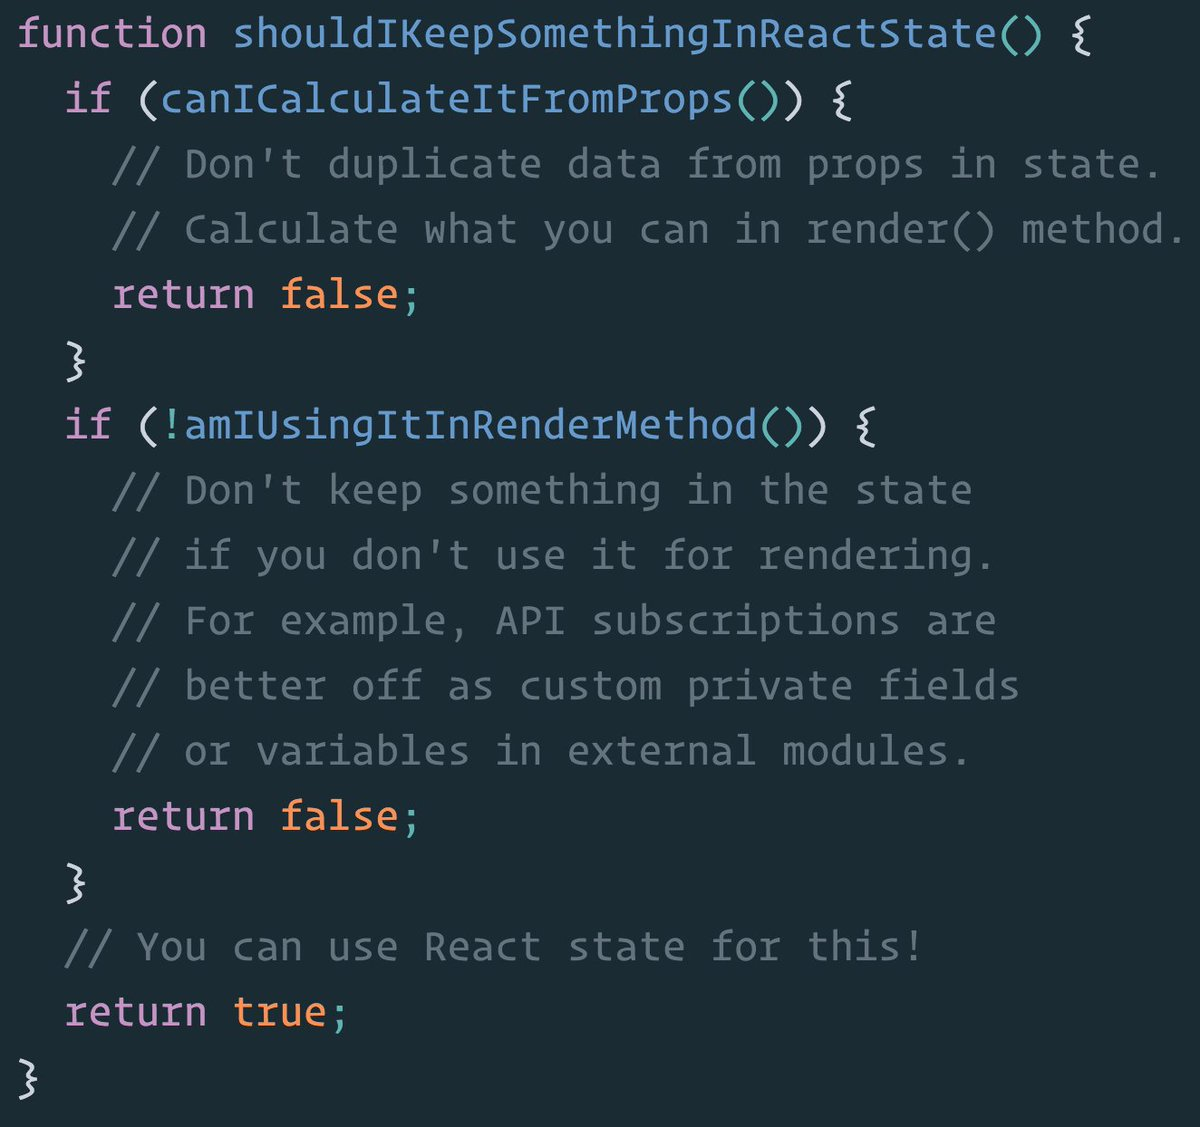
\includegraphics[width=.8\textwidth]{images/dan-cheat-sheet}
\end{figure}


\section{Prop types}

Мы ставим перед собой цель, создавать переиспользуемые компоненты, поэтому нам нужно описывать интерфейс этих компонент удобным для пользователей этих компонент образом.

React из коробки позволяет нам описывать, какие параметры ожидает компонент и простые правила валидации к ним. Привила позволяют указывать, какого типа данных должны быть параметры, а также являются ли параметры обязательными. Помимо этого React позволяет определять пользовательские функции проверки параметров.

Посмотрим на простой пример:

\begin{lstlisting}
const Button = ({ text }) => <button>{text}</button>
Button.propTypes = {
  text: React.PropTypes.string,
}
\end{lstlisting}

В этом примере мы создаем простую компонент-функцию, которая должна получать один параметр $text$, который должен быть типа $string$.

Теперь каждый, кто попытается воспользоваться данным компонентом, сможет легко понять, что ему нужно передавать даже без детального чтения кода.

Но что если компонент вообще не сможет работать, если ему не передать определенный параметр? В этом случае этот параметр можно указать как обязательный:

\begin{lstlisting}
Button.propTypes = {
  text: React.PropTypes.string.isRequired,
}
\end{lstlisting}

В этом случае кто-либо, кто создаст такой компонент, не передав обязательный параметр, получат следующую ошибку:

\begin{quotation}
\textbf{Failed prop type: Required prop `text` was not specified in `Button`.}
\end{quotation}

Важно понимать, что предупреждение об ошибке мы получим только в режиме разработки. В релизной сборке валидация с $propTypes$ выключается в целях улучшения производительности.

React предоставляет возможность проверки множества типов параметров: от чисел до массивов и компонент.

Если мы хотим, чтобы компонент работал с данными разных типов, передаваемых через один параметр, то можем использовать функцию \textbf{oneOf}, которая позволяет указать список разных типов для одного параметра.

Также стоит стараться передавать через параметры только примитивные типы, так как они лучше поддаются отладке и терстированию.

Передача примитивов также позволяет быстрее находить разбухающие интерфейсы у компонент. Если компонент начинает требовать все больше и больше параметров, то возможно он содержит больше логики чем должен и нарушает принцип единственности ответственности.

Если мы замечаем, что компонент получает множество параметров, которые слабо связаны логикой приложение, то можно попробовать разделить этот компонент на два независимых.

Однако нам все равно достаточно часто приходится передавать компонентам объекты. В этом случае для валидации следует использовать функцию $shape$.

Функция $shape$ позволяет определить параметр типа объект, а также определить тип всех полей, которые должны быть у этого объекта, которые в свою очередь тоже могут быть объектами.

Например, если мы создадим компонент $Profile$, который ожидает объект с именем и фамилией пользователя, то мы можем создать следующие $propTypes$:

\begin{lstlisting}
const Profile = ({ user }) =>(
  <div>{user.name} {user.surname}</div>
)
Profile.propTypes = {
  user: React.PropTypes.shape({
    name: React.PropTypes.string.isRequired,
    surname: React.PropTypes.string,
  }).isRequired,
}
\end{lstlisting}

Если же ни одного из стандартных методов валидации React нам не подходят, то мы можем определить собственную функцию проверки:

\begin{lstlisting}
user: React.PropTypes.shape({
  age: (props, propName) => {
    if (!(props[propName] > 0 && props[propName] < 100)) {
      return new Error(`${propName} must be between 1 and 99`)
    }
    return null
  },
})
\end{lstlisting}

Например, в примере выше мы проверяем, что возраст находится в определенном числовом промежутке. Если же возраст выйдет за этот промежуток, то мы увидим соответствующую ошибку в консоли.

\subsection*{React Docgen}

Хорошо описанные $propTypes$ уже значительное облегчение жизни тем, кто будет пользоваться нашими компонентами. Но мы можем пойти дальше и еще больше упростить их использование.

Когда количество компонентов значительно возрастает, то появляется проблема поиска необходимого компонента среди многих, особенно для новых членов проекта.

Но если мы поддерживали $propTypes$ в хорошем состоянии, то мы можем автоматически создавать из них документацию.

Для этого мы можем использовать библиотеку $react-docgen$, которую можно установить следующей командой:

\begin{lstlisting}
npm install --global react-docgen
\end{lstlisting}

React Docgen проходит по файлу с компонентом и достает, необходимую для него информацию, из $propTypes$ и комментариев.

Например, если у нас есть компонент:

\begin{lstlisting}
const Button = ({ text }) => <button>{text}</button>
Button.propTypes = {
  text: React.PropTypes.string,
}
\end{lstlisting}

И мы запустим:

\begin{lstlisting}
react-docgen button.js
\end{lstlisting}

Мы получим следующий результат;

\begin{lstlisting}
{
  "description": "",
  "methods": [],
  "props": {
    "text": {
      "type": {
        "name": "string" 
      },
      "required": false,
      "description": ""
    } 
  }
}
\end{lstlisting}

Этот JSON представляет собой описание интерфейса компонента. Как вы видите, в него попали поля и их типы, описанные в $propTypes$.

Также мы можем добавить комментарий к нашему компоненту:

\begin{lstlisting}
/**
 * A generic button with text.
 */
const Button = ({ text }) => <button>{text}</button>
Button.propTypes = {
  /**
   * The text of the button.
   */
  text: React.PropTypes.string,
}
\end{lstlisting}

Если мы снова запустим Docgen, то получим:

\begin{lstlisting}
{
  "description": "A generic button with text.",
  "methods": [],
  "props": {
    "text": {
      "type": {
        "name": "string"
      },
      "required": false,
      "description": "The text of the button."
    }
  }
}
\end{lstlisting}

Теперь, с этим описанием интерфейса в формате JSON мы можем создать документацию и использовать ее внутри команды.

Результат работы Docgen имеет простой формат, поэтому не составляет никакого труда создать страницу с документацией на его основе.

Один из ярких примеров использования React Docgen - документация библиотеки $Material UI$, где вся документация создана на основе исходного кода библиотеки.


\section{Переиспользуемые компоненты}

Мы уже хорошо разобрались с тем как создавать компоненты, как использовать внутреннее состояние компонент и как сделать их переиспользуемыми с помощью $propTypes$.

Давайте теперь, вооружившись всеми полученными знаниями, попробуем сделать из непереиспользуемыех компонент переиспользуемые.

Предположим, что у нас есть компонент, который загружает список постов через API сервера и отображает их на экране.

Это упрощенный пример, но он хорошо подходит, чтобы показать все этапы создания переиспользуемого компонента.

Создадим класс посредством его наследования от React.Component:

\begin{lstlisting}
class PostList extends React.Component
\end{lstlisting}

Затем создадим конструктор и добавим загрузку данных в $componentDidMount$:

\begin{lstlisting}
constructor(props) {
  super(props)
  this.state = {
    posts: [],
  } 
}
componentDidMount() {
  Posts.fetch().then(posts => {
    this.setState({ posts })
  })
}
\end{lstlisting}

Во $state$ компонента только одно поле $posts$, в котором мы будем хранить посты и которое инициализируется пустым массивом.

В $componentDidMount$ вызывается API сервера, для получения списка постов. По окончанию запроса посты сохраняются в $state$ компонента с помощью метода $setState$.

Это распространенный паттерн загрузки данных, другие варианты детальнее мы рассмотрим в Главе 5.

$Posts$ - это вспомогательный класс, который содержит логику общения с сервером. Сейчас для нас важно только то, что этот класс имеет метод $fetch$, который возвращает $Promise$, который при успешном выполнении вернет список постов.

Теперь мы можем отобразить список постов:

\begin{lstlisting}
render() {
  return (
    <ul>
      {this.state.posts.map(post => (
        <li key={post.id}>
          <h1>{post.title}</h1>
          {post.excerpt && <p>{post.excerpt}</p>}
        </li> ))}
    </ul> 
  )
}
\end{lstlisting}

Внутри метода $render$ мы обходим все посты и для каждого создаем элемент $<li>$.

Мы полагаем, что у поста всегда есть поле $title$ и безусловно показываем его внутри $<h1>$. Поле же $post.excerpt$ мы считаем необязательным и отображаем только при наличии.

Теперь представим другой компонент. Пусть он отображает список пользователей, которые получает из $props$, а не из собственного состояния:

\begin{lstlisting}
const UserList = ({ users }) => (
  <ul>
    {users.map(user => (
      <li key={user.id}>
        <h1>{user.username}</h1>
        {user.bio && <p>{user.bio}</p>}
      </li>
      )
    )} 
  </ul>
)
\end{lstlisting}

Данный компонент отображает список пользователей очень похожим на отображение постов способом.

Отличие в том, что теперь вместо $title$ отображается $username$ и опциональное поле теперь $bio$ пользователя вместо $excerpt$ поста. 

Дублирующийся код как правило считаются плохим звоночком, так что давайте разбираться как React позволяет следовать правилу \textbf{Не повторяйся (Don't Repeat Yourself, DRY)}. Прежде всего мы можем создать отдельный компонент $List$, в который вынесем логику отображения списков, отделив ее от самих данных. Главным требованием является возможность передать ключи полей по которым мы сможем получить данные, чтобы иметь возможность брать нужные данные из разных типов объектов.

Чтобы сделать это, мы определим два параметра: $titleKey$ для передачи ключа, по которому мы получим значение для  обязательного поля, и $textKey$ для передачи ключа опционального поля.

Параметры нашего нового компонента будут выглядеть следующим образом:

\begin{lstlisting}
List.propTypes = {
  collection: React.PropTypes.array,
  textKey: React.PropTypes.string,
  titleKey: React.PropTypes.string,
}
\end{lstlisting}

Так как $List$ не будет обладать своим собственным состоянием, мы можем его создать как компонент-функцию:

\begin{lstlisting}
const List = ({ collection, textKey, titleKey }) => (
  <ul>
    {collection.map(item =>
      <Item
        key={item.id}
        text={item[textKey]}
        title={item[titleKey]}
      /> 
    )}
  </ul> 
)
\end{lstlisting}

Компонент $List$ получает через $props$ коллекцию объектов, проходит по ним и преобразует в элементы $Item$, который мы скоро реализуем. Также в дочерний элемент мы передаем $text$ и $title$, который получаем с помощью полученных ключей из элементов коллекции.

Компонент $Item$ будет максимально простым и чистым:

\begin{lstlisting}
const Item = ({ text, title }) => (
  <li>
    <h1>{title}</h1>
    {text && <p>{text}</p>}
  </li>
)

Item.propTypes = {
  text: React.PropTypes.string,
  title: React.PropTypes.string,
}
\end{lstlisting}

Таким образом мы создали два компонента с достаточно простыми интерфейсами, чтобы с их помощью отображать пользователей, посты или что-либо еще. При этом такие небольшие компоненты очень удобны в поддержке и тестировании.

Отлично, теперь мы можем переписать наши исходные компоненты с использованием новых вспомогательных компонент.

Метод $render$ компонента $PostsList$ будет выглядеть следующим образом:

\begin{lstlisting}
render() {
  return (
    <List
      collection={this.state.posts}
      textKey="excerpt"
      titleKey="title"
    />
  )
}
\end{lstlisting}

А компонент-функция $UserList$ следующим:

\begin{lstlisting}
const UserList = ({ users }) => (
  <List
    collection={users}
    textKey="bio"
    titleKey="username"
  /> 
)
\end{lstlisting}

Таким образом мы из узкоспециализированных компонент получили базовые компоненты, которые могут быть переиспользованы в будущем.

Мы также можем использовать $react-docgen$ для генерации документации для полученных нами компонент.

Также теперь в случае необходимости расширения данного отображения, которое пока состоит из двух текстовых полей, нам будет достаточно поменять его в одном компоненте $Item$, а не в множестве узкоспециализированных компонент.

Например, если нам понадобится в случае слишком длинной строки урезать ее и показывать троеточие, нам будет достаточно добавить эту логику внутрь одного компонента.

\section{Living style guides}

Использование переиспользуемых компонент с простыми интерфейсами - хороший способ сократить количество дублирующегося кода в проекте, но это не единственная причина, чтобы сосредоточиться на переиспользуемости.

Если вы создаете простые и понятные компоненты с чистыми интерфейсами, которые хорошо отделены абстракциями от конкретных данных, то эти компоненты можно объединить в библиотеку компонент и использовать за пределами команды. Такая библиотека будет представлять из себя набор готовых к использованию блоков, которыми можно будет поделиться с другими командами, дизайнерами или выложить ее в open source.

Очень часто новым членам команды может быть сложно понять, какие компоненты уже есть, а какие нужно реализовать. Решением этой проблемы может быть создание Style guide'а, которое бы позволило распространять не только сами компоненты, но и примеры их использования.

По сути style guide - это собранное визуальное представление всех единичных компонентов, которые уже реализованы в проекте. Это очень удобный способ сохранять единый стиль всех компонент среди множества разработчиков разного уровня. 

К сожалению, создание style guide'а не всегда является простой задачей, так как из-за меняющихся требований может появиться множество дублирующихся компонент с небольшими отличиями, решающие какие-то локальные проблемы. Тем не менее React позволяет без значительных усилий создавать такой род документации, что может окупить немало времени в будущем.

Но не только React может вам помочь создать библиотеку визуальных компонентов из кода самих компонент. Есть инструменты, которые помогают решить эту проблему, один из которых $react-storybook$.

React Storybook изолирует компоненты, предоставляя вам возможность создавать компоненты без запуска всего приложения, что помогает в тестировании и разработке.

Как видно из названия библиотеки React Storybook позволяет создавать истории для отображения разных состояний компонента. Например, если вы пишите TO-DO приложение, то вы можете создать две истории для отображения выбранного и невыбранного состояний элемента.

Давайте попробуем применить эту библиотеку к примеру с компонентом $List$. Прежде всего нам нужно установить Storybook:

%npm install --save @kadira/react-storybook-addon

Теперь мы можем начать создавать истории.

В нашем примере компонент $Item$ требует обязательный параметр $title$ и опциональный $text$, в этом случае мы можем создать как минимум две истории.

Обычно истории хранят в директории $stories$ внутри проекта, но в целом никто не запрещает использовать любую удобную для вас директорию.

Внутри этой директории можно создать специально файл для каждой из компонент.

В нашем случае создадим файл $list.js$. В этом файле обязательно необходимо добавить импорт основной функции библиотеки:

\begin{lstlisting}
import { storiesOf } from '@kadira/storybook'
\end{lstlisting}

Дальше мы можем создать истории следующим образом:

\begin{lstlisting}
storiesOf('List', module)
  .add('without text field', () => (
    <List collection={posts} titleKey="title" />
  ))
\end{lstlisting}

Функция $storiesOf$ принимает аргументом название компонента и позволяет добавить для него множество историй. Каждая история включает в себя описание и функцию, которая создает необходимый компонент.

В нашем случае $posts$ может быть объектом вида:

\begin{lstlisting}
const posts = [
  {
    id: 1,
    title: 'Create Apps with No Configuration',
  },
  {
    id: 2,
    title: 'Mixins Considered Harmful',
  },
]
\end{lstlisting}

Перед запуском Storybook и создания нашей визуальной коллекции нам необходимо настроить библиотеку. Для этого необходимо создать директорию $.storybook$. 

Внутри этой директории нам нужно создать файл $config.js$ для загрузки наших историй:

\begin{lstlisting}
import { configure } from '@kadira/storybook'
function loadStories() {
  require('../src/stories/list')
}
configure(loadStories, module)
\end{lstlisting}

Сначала мы загружаем функцию $configure$ из библиотеки, а затем описываем функцию для загрузки историй по путям к их файлам.

И последний шаг, если мы хотим, чтобы storybook с нашими компонентами был доступен из браузера, мы можем добавить специальный скрипт в package.json:

\begin{lstlisting}
"storybook": "start-storybook -p 9001"
\end{lstlisting}

Теперь мы можем запустить storybook:

\begin{lstlisting}
npm run storybook
\end{lstlisting}

И открыть в браузере $http://localhost:9001$.

Теперь мы можем увидеть интерфейс storybook. Слева находится список наших историй. Если мы нажмем на историю, то справа увидим соответствующий ей компонент.

Отлично, теперь у нас есть визуальная документация наших компонент, чтобы все члены команды, в том числе продуктовые менеджеры и дизайнеры, имели представление о существующей базе готовых компонентов.

В завершение мы можем создать еще одну историю.

Наш лист умеет отображать элементы с $title$ и $text$, поэтому добавим второй атрибут в список постов:

\begin{lstlisting}
const posts = [
  {
    id: 1,
    title: 'Create Apps with No Configuration',
    excerpt: 'Create React App is a new officially supported...',
  }, 
  {
    id: 2,
    title: 'Mixins Considered Harmful',
    excerpt: '"How do I share the code between several...',
  }
]
\end{lstlisting}

После этого добавим еще одну историю, где передадим оба параметра:

\begin{lstlisting}
.add('with text field', () => (
  <List collection={posts} titleKey="title" textKey="excerpt" />
))
\end{lstlisting}

Если мы сейчас вернемся в браузер, то увидим, что наша страница автоматически обновилась, и добавилась вторая история.

Таким образом для сложных компонентов мы можем добавить любое количество историй, чтобы показать все состояния, в которых они могут находиться.

\section{Заключение}

Поздравляю, мы разобрались с созданием переиспользуемых компонент.

В этой главе мы детально посмотрели как можно создавать компоненты и в чем различие между компонент-функциями и компонентами с внутренним состоянием. Также мы изучили как осуществляется изменение состояния React компонент и как это приводит к перерисовке компонента. Помимо этого мы посмотрели как описывать параметры компонента и как это помогает в совместной работе надо общими элементами.

И в конце мы посмотрели на примеры превращения узкоспециализированных компонент в переиспользуемые посредством вынесения общей логики в достаточно абстрактные базовые компоненты.

Теперь пришло время посмотреть на разные техники комбинации компонентов между собой.


